% \begin{table}[]
%     \centering
%     \begin{tabular}{llll}
%     \toprule
%     Number & First author & Year & Citation\\
%     \midrule
%       1  &  PENG & 2002 & \cite{peng2004semiquantitative}  is 2004 \\
%       2  &  SATON  2002    is SATOH &2002 &\cite{satoh2002identification} \\
%     3 &  SCHWENK & 2013 &  \cite{schwenk2012high} 2012\\
%     4 &  SELIMI  & 2009 & \cite{selimi2009proteomic} \\
%     5 &  TRINIDAD & 2005& \cite{trinidad2005phosphorylation} \\  
% 6& TRINIDAD  &2008 & \cite{trinidad2008quantitative} \\
% 7&  WALIKONIS & 2000&  \cite{walikonis2000identification}\\ 
%  8 &YOSHIMURA &2004& \cite{yoshimura2004molecular}   \\
% 9 &FROMER &2014 & \footnote{Not in Heil I only find fromer in an oksana paper on PSD and it is on scz I assume this is Focking and the one cited in Heil is bipolar
% and they have 2033} PSD proteins Focking \cite{focking2016proteomic}\\
% 10&FARR &2004 &  \cite{farr2004proteomic}\\
% 11&Distler.PSDII & 2014 &\cite{distler2014depth}\\
% 12& BAYES & 2011&    \cite{bayes2011characterization}  \\
% 13 &  BAYES &2012 & \cite{bayes2012comparative}  \\  
% 14& COLLINS &2006 & \cite{collins2006molecular}\\
% 15 & DOSEMECI  &2007&  \cite{dosemeci2007composition}\\
% 16 & FERNANDES  &2009&  \cite{fernandez2009targeted}\\
% 17 & BAYES &2014 &  \cite{bayes2014human}\\
% \bottomrule
%     \end{tabular}
%     \caption[Primary proteomic studies contributing to the PSP graph]{Primary proteomic studies contributing to the PSP graph \footnote{to Douglas: if using the Oksana Clean Published data TO REMOVE please see note on text}}
%     \label{tab:oksana clean published}
% \end{table}


\begin{table}[]
    \centering
    \begin{tabular}{llllllll}
    \toprule
     & First author & Year & Reference & Region & Species & $n$ & In Oksana file \\
    \midrule
1 &    WALIKONIS &2000 &Walikonis et al. (2000)\cite{walikonis2000identification} &postsynapse & rat & 29 \\
2 &PENG&2004&Peng et al. (2004) \cite{peng2004semiquantitative}&postsynapse& rat& 325\\
3 &SATOH&2002&Satoh et al. (2002)\cite{satoh2002identification} &postsynapse &mouse &45\\
4 &YOSHIMURA&2004&Yoshimura et al. (2004) \cite{yoshimura2004molecular} &postsynapse& rat &435\\
5 &FARR&2004&Farr et al. (2004)  \cite{farr2004proteomic}&postsynapse &rat &71 &Yes\\
6 &JORDAN&2004&Jordan et al. (2004)&postsynapse &mouse and rat &390& NOT\\
7&LI&2004 &wan Li et al. (2003)&postsynapse &rat& 137& NOT\\
8&TRINIDAD&2005 &Trinidad et al. (2005) \cite{trinidad2005phosphorylation}&postsynapse&mouse& 234& YES\\
9&CHENG&2006&Cheng et al. (2006)&postsynapse& rat& 288& NO\\
10&COLLINS&2006&Collins et al. (2006)\cite{collins2006molecular}&postsynapse &mouse& 717& YES\\
11&DOSEMESI&2006&Dosemeci et al. (2006)&postsynapse& rat& 113& NO\\
12&DOSEMESI&2007&Dosemeci et al. (2007)&postsynapse& rat& 548& YES\\
13&TRINIDAD&2008&Trinidad et al. (2008)&postsynapse& mouse& 2150& YES\\
14&SELIMI&2009&Selimi et al. (2009)\cite{selimi2009proteomic}&postsynapse &mouse &61& YES\\
15&FERNANDEZ&2009&Fernández et al. (2009)  \cite{fernandez2009targeted}&postsynapse& mouse &292& YES\\
16&BAYES&2010&Bayés et al. (2011)&postsynapse &human &1441& YES\\
17&BAYES&2012&Bayés et al. (2012)&postsynapse &mouse &1545 &YES\\
18&SCHWENK&2012&Schwenk et al. (2012) \cite{schwenk2012high}&postsynapse &unknown &34& YES\\
19&DISTLER PSD1*&2014&Distler et al. (2014)&postsynapse& mouse& 3545& NO \footnote{intended per email}\\
20&DISTLER PSD2*&2014&Distler et al. (2014)&postsynapse& mouse& 2092*& Oksana\\
21&BAYES&2014&Bayés et al. (2014)&postsynapse& human &1141& YES\\
22&UEZU&2016&Uezu et al. (2016)&postsynapse &mouse &1111 &NO\\
23&FOCKING&2016&Föcking et al. (2016)&postsynapse& human &2026 &NO\\
\bottomrule
    \end{tabular}
    \caption[Primary Proteomic studies appearing in PSP cleaned from Heil (2018)]{Primary proteomic studies contributing to the PSP take from Heil 2018\cite{heil2018systems} from Katharina PhD p84 table 5.1. \footnote{to Douglas: These should have been the same as given to me as per email from Colin need to chose one see note on text. Distler PSD1 is definitely dropped from the cleaned data. The graph is somewhere between these two points. The most conservative is the Oksana one.}}
    \label{tab:Katharina_phd_studiesFF}
\end{table}
% \section{NOT IN DOCUMENT}
% \section{FRAMEWORK FOR GSA - USED}
% %%% FRAMEWORK
% \section{Gene Ontology Analysis of MAGMA genes FRAMEWORK}
% They are not all measured the same way eg DEPICT in Okbay so worth going through 

% Is the gtex higher in both education
%     \subsection{Intelligence Replication}
%         \subsubsection{Authors findings}
%         MAGMA Regulating cell development $P=3.5 \times 10^{-6}$. Authors state that several (?14) of the significant genes are more expressed in the CNS.
%         \subsubsection{Ontology ORA Genome}
%         \paragraph{Toppgene ToppFun Intelligence Replication}
%         \subparagraph{ToppFun BP} nil
%         \subparagraph{ToppFun MF} nil
%         \subparagraph{ToppFun CC} See table~\ref{tab:cellular component in toppgene}
%         \begin{table}[ht]
%     \centering
%     \begin{tabular}{llllllll}
%          ID &Name 	&	pValue 	&FDR BH &	FDR BY 	&Bonferroni  	&n input & n annot  \\
%          GO:0032584 &	growth cone membrane\footnote{part of growth cone: distal axon: neuron projection:cell projection: cellular anatomical entity} &		1.416E-4 &	3.838E-2 &2.373E-1&	3.838E-2 &	2 &	8 \\
%     \end{tabular}
%     \caption{Cellular component in toppgene}
%     \label{tab:cellular component in toppgene}
% \end{table}
%         \paragraph{Panther Intelligence Replication}
%         All genes 47 identified
        
%         \subparagraph{Panther BP} nil
%         \subparagraph{Panther MF} nil
%         \subparagraph{Panther CC} Two terms Cytoplasm GO:0005737 n in annotation 11714 n in set	40; expected 	26.40 ; fold change	1.51 ;	+ 	; raw P4.29E-05 	; FDR 0.431 4.31E-02 and its parent term intracellular GO:0005622 n in annotation 14693 ; n in set	45 ; E	33.12 ; fold	1.36 ;	+ ;	3.24E-05 ; FDR	6.50E-02 Not significant


%         \subsubsection{Ontology ORA Synaptic}
        
%         \subsubsection{Others}
%         \begin{itemize}
%             \item path to code
%             \item GTex
%             \item Other phenotypes
%         \end{itemize}
        

%     \subsection{Education Replication}
%         \subsubsection{Authors findings Education Replication}
%         Pathways involving CNS development
%         13 Gtex tissues in CNS showed elevated expression of genes near EduYears SNPs
%         283 Gene sets. 5 clusters ``neural progenitor cells, migration of new neurons to cortex, projection of axons to target, sprouting of dendrites and spines and neuronal signalling and synaptic plastigcity throughout the lifespan'' not precis quote but close last group is the one of interest to use 
%         Genes prioritised by DEPICT. Overlap with ID and ASD.GRIK2<10e-6, CALM2 < 10e-4 PPI in Figure 3 ?includes multiple testing. 685 genes at 273 Loci p 88 of supplemental material supplementary table 4.1 wherever that is. We have not used this approach as \url{https://github.com/perslab/gwas-snps-loci} as predominant approach is MAGMA.
%         \subsubsection{Ontology ORA Education Replication Genome}
%       \paragraph{toppgene}
%           \subparagraph{BP toppgene}  See table~\ref{tab:BP EA2 all significant toppgene} 
%             \begin{table}[ht]
% \centering
% \begin{tabular}{rllrrrr}
%   \hline
%  & ID & Name & test & Genome & p & Bon \\ 
%   \hline
% 1 & GO:0022008 & neurogenesis & 26 & 1866 & $5.97 \times 10^{-7}$ & 0.00176 \\ 
%   2 & GO:0042063 & gliogenesis & 11 & 352 & $1.14 \times 10^{-6}$ & 0.00337 \\ 
%   3 & GO:0007417 & central nervous syst & 19 & 1129 & $1.81 \times 10^{-6}$ & 0.00535 \\ 
%   4 & GO:0048666 & neuron development & 20 & 1297 & $3.53 \times 10^{-6}$ & 0.01041 \\ 
%   5 & GO:0010001 & glial cell different & 9 & 261 & $5.16 \times 10^{-6}$ & 0.01522 \\ 
%   6 & GO:0050808 & synapse organization & 12 & 498 & $5.39 \times 10^{-6}$ & 0.01589 \\ 
%   7 & GO:0048667 & cell morphogenesis i & 14 & 688 & $5.92 \times 10^{-6}$ & 0.01747 \\ 
%   8 & GO:0048699 & generation of neuron & 23 & 1751 & $8.43 \times 10^{-6}$ & 0.02489 \\ 
%   9 & GO:0048812 & neuron projection mo & 14 & 742 & $1.39 \times 10^{-5}$ & 0.04100 \\ 
%   10 & GO:0010771 & negative regulation  & 6 & 109 & $1.53 \times 10^{-5}$ & 0.04527 \\ 
%   \hline
% \end{tabular}
% \caption{BP EA2 all significant Toppgene 99 genes in total \url{source('~/RProjects/paper_xls_output/R/chapter_2/eda_toppgene_all_significant_ea2.R')}} 
% \label{tab:BP EA2 all significant toppgene}
% \end{table}

% \subparagraph{CC toppgene}
% See table~\ref{tab:CC EA2 all significant Toppgene}
% % latex table generated in R 3.6.3 by xtable 1.8-4 package
% % Wed Aug 19 12:29:17 2020
% \begin{table}[ht]
% \centering
% \begin{tabular}{llrrrr}
%   \hline
% ID & Name & test & Genome & p & Bon \\ 
%   \hline
% GO:0098794 & postsynapse & 16 & 825 & $1.46 \times 10^{-6}$ & 0.00050 \\ 
%   GO:0045202 & synapse & 20 & 1482 & $1.58 \times 10^{-5}$ & 0.00547 \\ 
%   \hline
% \end{tabular}
% \caption{CC EA2 all significant Toppgene \url{source('~/RProjects/paper_xls_output/R/chapter_2/eda_toppgene_all_significant_ea2.R')} }
% \label{tab:CC EA2 all significant Toppgene}
% \end{table}


        
%     \paragraph{panther}
%     Panther by default uses HGNC numerical symbols so it is necessary to prefix Entrez ID with GeneID: this is done in a custom R script \url{source('~/RProjects/paper_xls_output/R/chapter_2/exploratory_data_analysis.R')}
%     Unmapped Gene ID using entrez with Gene ID prefix
%     GeneID:246744

%         \subparagraph{BP Panther}
%         BP panther ordered by FDR 19 items top Nervous system development FDR 0.006 (2430 genes in reference) 2.57 fold change (see table~\ref{tab:GO.biological.process.complete Panther Gene Ontology Enrichment significant genes in Education Replication}). The heirarchy of terms in gene ontology is shown in figure~\ref{fig:panther GO Biological Process Heirarchy shown}\footnote{Douglas: I have included this as a screenshot. Parsing the xml and getting it into latex took longer than I thought so I went straight to screenshot as a last resort could do the indentation by hand. Thought worth showing (as DEPICT, MAGMA etc as far as I can see ignore heirarchy) but interested in what you thought. The standard table output for panther doesn't have the heirarchy.}
        
%         \begin{figure}
%             \centering
%             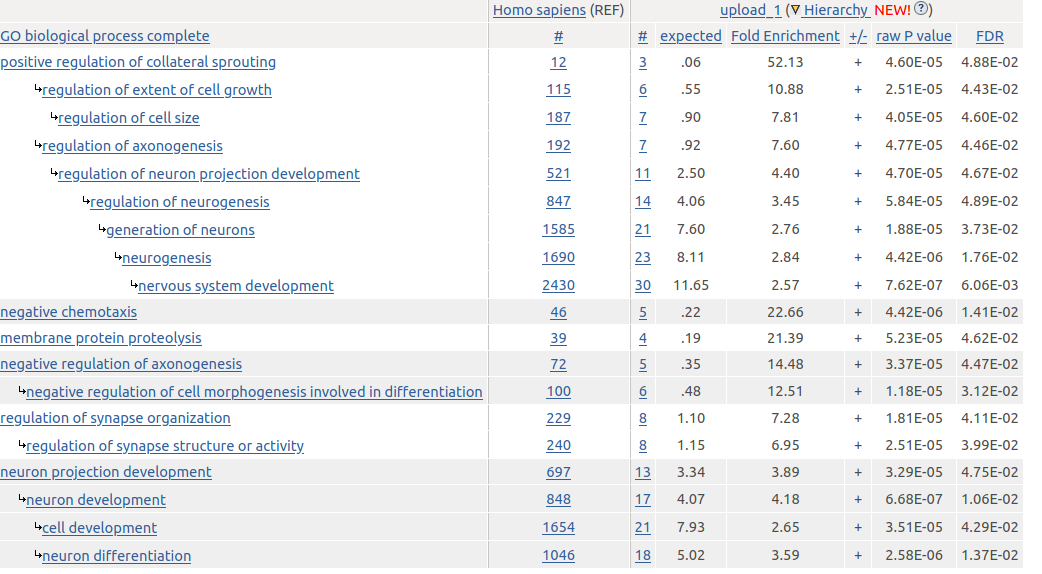
\includegraphics[width=\textwidth]{images/screenshots/EA2_BP_Panther_all_genes.png}
%             \caption{Panther GO Biological Process EA2 Hierarchy shown. This includes all genes accessed by manually editing the Gene Symbol}
%             \label{fig:panther GO Biological Process Heirarchy shown}
%         \end{figure}
%         % latex table generated in R 3.6.3 by xtable 1.8-4 package
% % Sun Aug 23 11:12:46 2020
% \begin{table}[ht]
% \centering
% \begin{tabular}{lrrrlrcc}
%   \hline
% GO.biological.process.complete & ref & test & [E] & ou & fold & P & FDR \\ 
%   \hline
% nervous system development (GO:0007399) & 2430 & 30 & 11.7 & + & 2.57 & $7.62 \times 10^{-7}$ & 0.006 \\ 
%   neuron development (GO:0048666) & 848 & 17 & 4.1 & + & 4.18 & $6.68 \times 10^{-7}$ & 0.011 \\ 
%   neuron differentiation (GO:0030182) & 1046 & 18 & 5.0 & + & 3.59 & $2.58 \times 10^{-6}$ & 0.014 \\ 
%   negative chemotaxis (GO:0050919) & 46 & 5 & 0.2 & + & 22.66 & $4.42 \times 10^{-6}$ & 0.014 \\ 
%   neurogenesis (GO:0022008) & 1690 & 23 & 8.1 & + & 2.84 & $4.42 \times 10^{-6}$ & 0.018 \\ 
%   \makecell{negative regulation of cell morphogenesis\\ involved in differentiation (GO:0010771)} & 100 & 6 & 0.5 & + & 12.51 & $1.18 \times 10^{-5}$ & 0.031 \\ 
%   generation of neurons (GO:0048699) & 1585 & 21 & 7.6 & + & 2.76 & $1.88 \times 10^{-5}$ & 0.037 \\ 
%   regulation of synapse structure or activity (GO:0050803) & 240 & 8 & 1.1 & + & 6.95 & $2.51 \times 10^{-5}$ & 0.040 \\ 
%   regulation of synapse organization (GO:0050807) & 229 & 8 & 1.1 & + & 7.28 & $1.81 \times 10^{-5}$ & 0.041 \\ 
%   cell development (GO:0048468) & 1654 & 21 & 7.9 & + & 2.65 & $3.51 \times 10^{-5}$ & 0.043 \\ 
%   regulation of extent of cell growth (GO:0061387) & 115 & 6 & 0.6 & + & 10.88 & $2.51 \times 10^{-5}$ & 0.044 \\ 
%   regulation of axonogenesis (GO:0050770) & 192 & 7 & 0.9 & + & 7.60 & $4.77 \times 10^{-5}$ & 0.045 \\ 
%   negative regulation of axonogenesis (GO:0050771) & 72 & 5 & 0.3 & + & 14.48 & $3.37 \times 10^{-5}$ & 0.045 \\ 
%   regulation of cell size (GO:0008361) & 187 & 7 & 0.9 & + & 7.81 & $4.05 \times 10^{-5}$ & 0.046 \\ 
%   membrane protein proteolysis (GO:0033619) & 39 & 4 & 0.2 & + & 21.39 & $5.23 \times 10^{-5}$ & 0.046 \\ 
%   regulation of neuron projection development (GO:0010975) & 521 & 11 & 2.5 & + & 4.40 & $4.70 \times 10^{-5}$ & 0.047 \\ 
%   neuron projection development (GO:0031175) & 697 & 13 & 3.3 & + & 3.89 & $3.29 \times 10^{-5}$ & 0.048 \\ 
%   positive regulation of collateral sprouting (GO:0048672) & 12 & 3 & 0.1 & + & 52.13 & $4.60 \times 10^{-5}$ & 0.049 \\ 
%   regulation of neurogenesis (GO:0050767) & 847 & 14 & 4.1 & + & 3.45 & $5.84 \times 10^{-5}$ & 0.049 \\ 
%   \hline
% \end{tabular}
% \caption{GO.biological.process.complete Panther Gene Ontology Enrichment significant genes in Education Replication} 
% \label{tab:GO.biological.process.complete Panther Gene Ontology Enrichment significant genes in Education Replication}
% \end{table}
%             \subparagraph{MF panther} No significant
%             \subparagraph{CC panther} Only one term synapse GO:0045202 1382 terms in reference 19 in table expected 6.50 fold enrichment 29.93 raw P $2.29\times 10^{-5}$ FDR 0.0459

%         Compare with toppgene widely variant scores noted in \cite{rhee2008use} and detailed discussion in \cite{khatri2005ontological}
%          \subsubsection{Ontology ORA Synaptic}
%          \subsubsection{Others}
%          \paragraph{disease enrichment}
%          Enrichment in DisGeNNet BeFree searched by toppfun of Intellectual disability
%         ID C3714756 	Intellectual Disability ; Source	DisGeNET BeFree ; p 	8.884E-7 ; FDR BH	1.648E-3; FR BY 	1.386E-2 ;Bonferroni	2.237E-3; Input 	20 	Total 1219
        
%         % latex table generated in R 3.6.3 by xtable 1.8-4 package
% % Sun Aug 23 12:35:02 2020
% \begin{table}[ht]
% \centering
% \begin{tabular}{rllr}
%   \hline
% Entrez.Gene.ID & Gene.Symbol & Gene.Name & Original.Symbol \\ 
%   \hline
% 5144 & PDE4D & phosphodiesterase 4D & 5144 \\ 
%   5662 & PSD & pleckstrin and Sec7 domain containing & 5662 \\ 
%   4137 & MAPT & microtubule associated protein tau & 4137 \\ 
%   4208 & MEF2C & myocyte enhancer factor 2C & 4208 \\ 
%   4744 & NEFH & neurofilament heavy & 4744 \\ 
%   257194 & NEGR1 & neuronal growth regulator 1 & 257194 \\ 
%   \hline
% \end{tabular}
% \caption{Intellectual disability genes significant in EA2 found in PSP} 
% \label{tab:Intellectual disability genes significant in EA2 found in PSP}
% \end{table}
%         Path to code
        
%         GTEx
% \clearpage



